\chapter{Implementacija i korisničko sučelje}
		
		
		\section{Korištene tehnologije i alati}
		
			\textbf{\textit{dio 2. revizije}}
			
			 \textit{Detaljno navesti sve tehnologije i alate koji su primijenjeni pri izradi dokumentacije i aplikacije. Ukratko ih opisati, te navesti njihovo značenje i mjesto primjene. Za svaki navedeni alat i tehnologiju je potrebno \textbf{navesti internet poveznicu} gdje se mogu preuzeti ili više saznati o njima}.
			
			
			\eject 
		
	
		\section{Ispitivanje programskog rješenja}
			
			U ovom poglavlju usredotočili smo se na testiranje programskog rješenja testirajući cijeli sustav, ali i komponente istog. Tijekom ispitivanja komponenti sustava korišteni su JUnit za izvršavanje testova te Mockito za stvaranje mock objekata korištenih u testiranju. Selenium IDE korišten je u ispitivanju sustava te nam je omogućio brzo i precizno provjeravanje funkcionalnosti web aplikacije.
			
			\subsection{Ispitivanje komponenti}
			
			U poglavlju o ispitivanju komponenti, razvijeni su i izvršeni testovi kako bi se osigurala kvaliteta i funkcionalnost komponenata sustava, a istovremeno se time osigurava pouzdanost i održivost koda. U nastavku su prikazani primjeri nekoliko testova koji su implementirani kao dio ispitivanja komponenti sustava:

			\textbf{Test sortiranja i ispisivanja događaja} provjerava ispravnu funkcionalnost sortiranja događaja prema određenom filtru, u ovom slučaju prema vremenu početka događaja. Također testirano je izlistavanje događaja, je li broj događaja jednak očekivanom broju. Korišten je JUnit za pisanje i izvršavanje testova te Mockito za stvaranje mock objekta i postavljanje očekivanja.


			\textbf{Test registracije korisinika} ispituje uspješnost registracije korisnika. Također se koriste Mock objekti koji simuliraju ponašanje komponenti tijekom registracije. Prikazana su dva testa, u jednom se testira registracija koja je uspješa, u drugom se testira neuspješna registracija korisnika.

			U nastavku su još prikazani sljedeći testovi: \textbf{Test slanja e-maila}, \textbf{Test spremanja recenzije}, \textbf{Test spremanja zainteresiranosti}. Oni redom provjeravaju točnost slanja e-maila, ispravnu funkcionalnost spremanja recenzije i zainteresiranosti. U navedenim testovima se također koriste spomenute tehnologije za provjeravanje ispravnosti. Osim testova, prikazano je i njihovo izvođenje te rezultat izvođenja.
			
			\begin{figure}[H]
				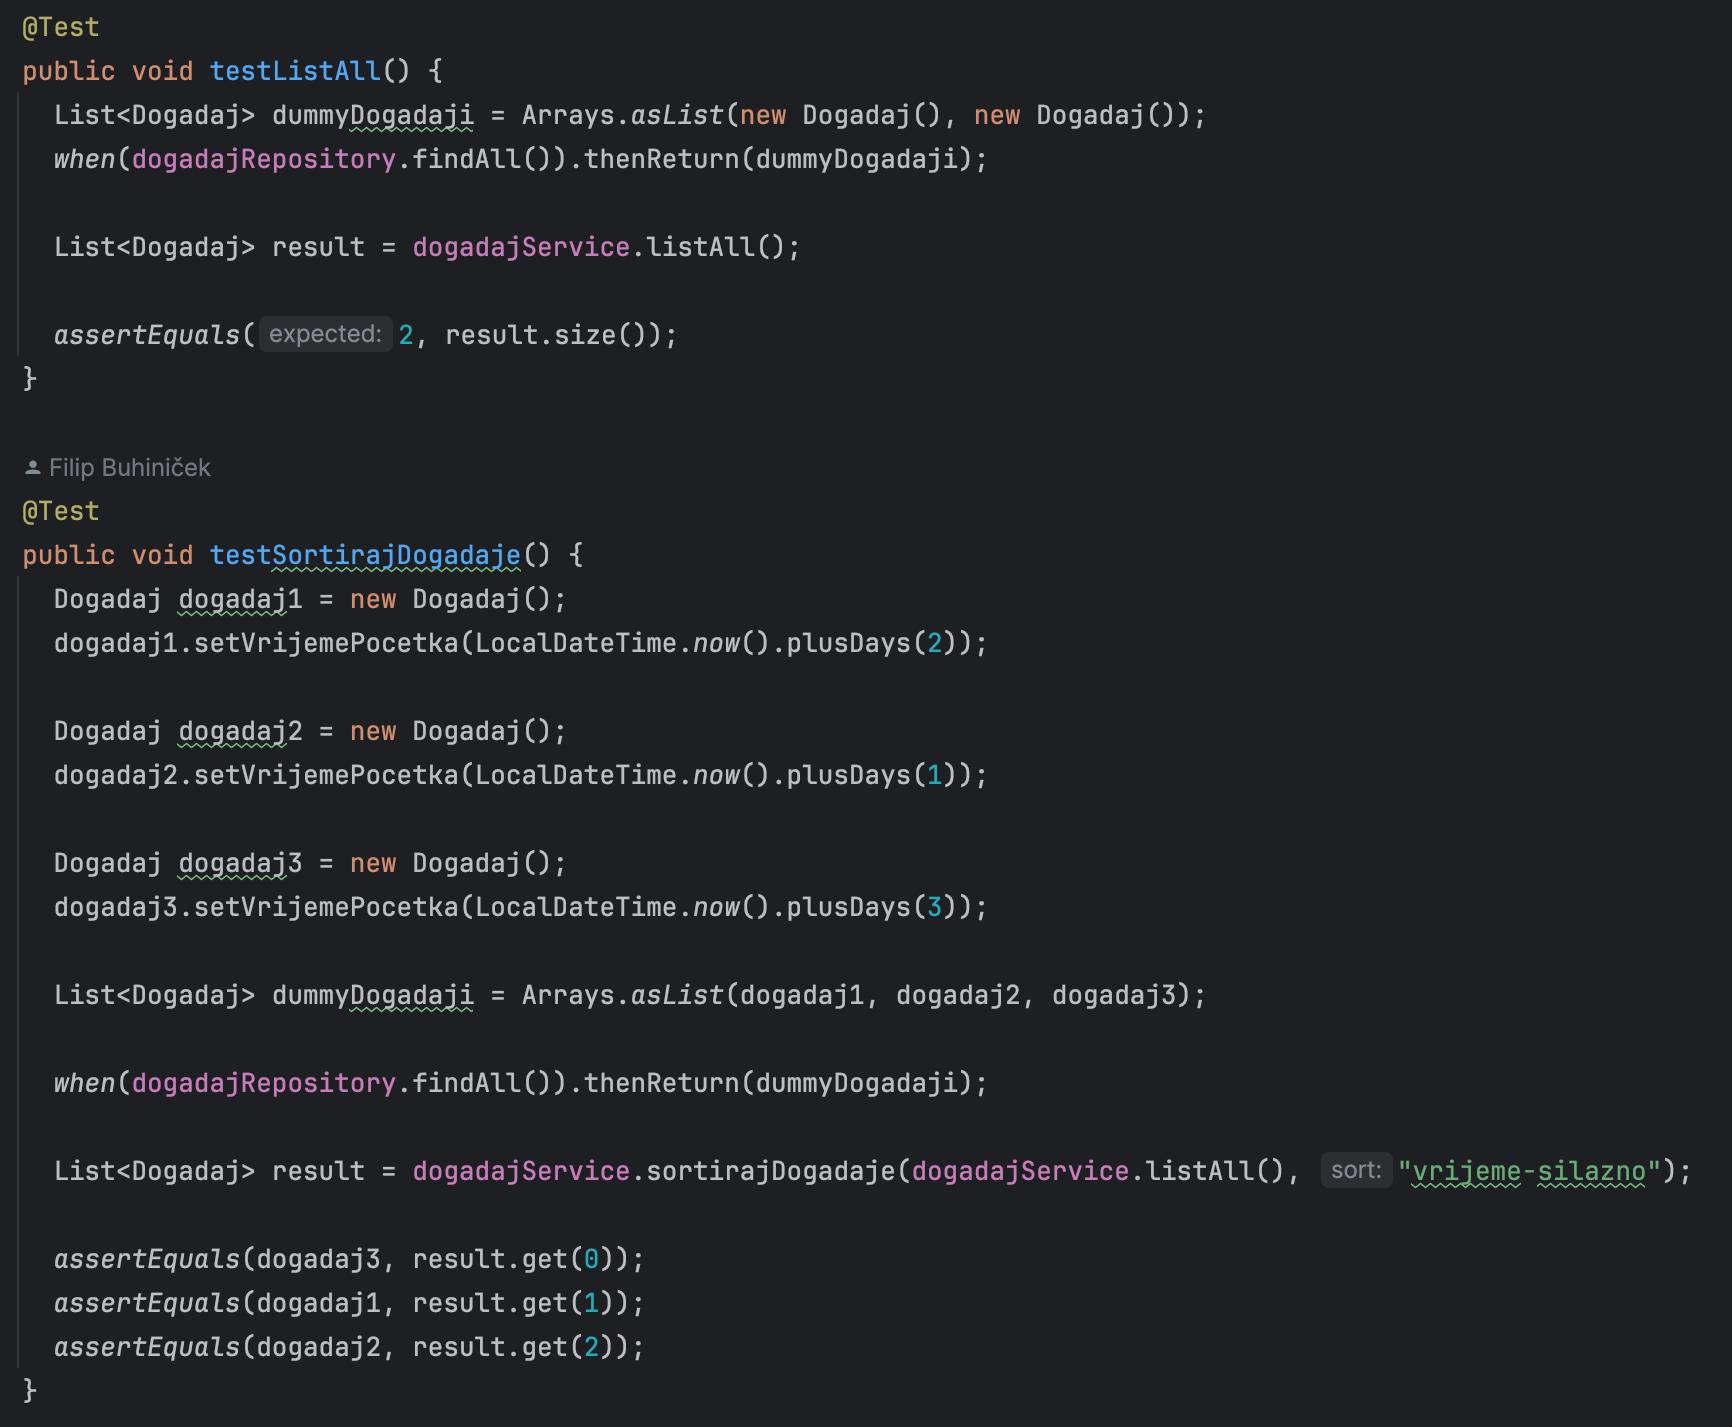
\includegraphics[scale=0.45]{testovi/dogadajTest.png}
				\centering
				\caption{Test za sortiranje i ispisivanje događaja}
				\label{fig:promjene}
			\end{figure}
			
			
			\begin{figure}[H]
				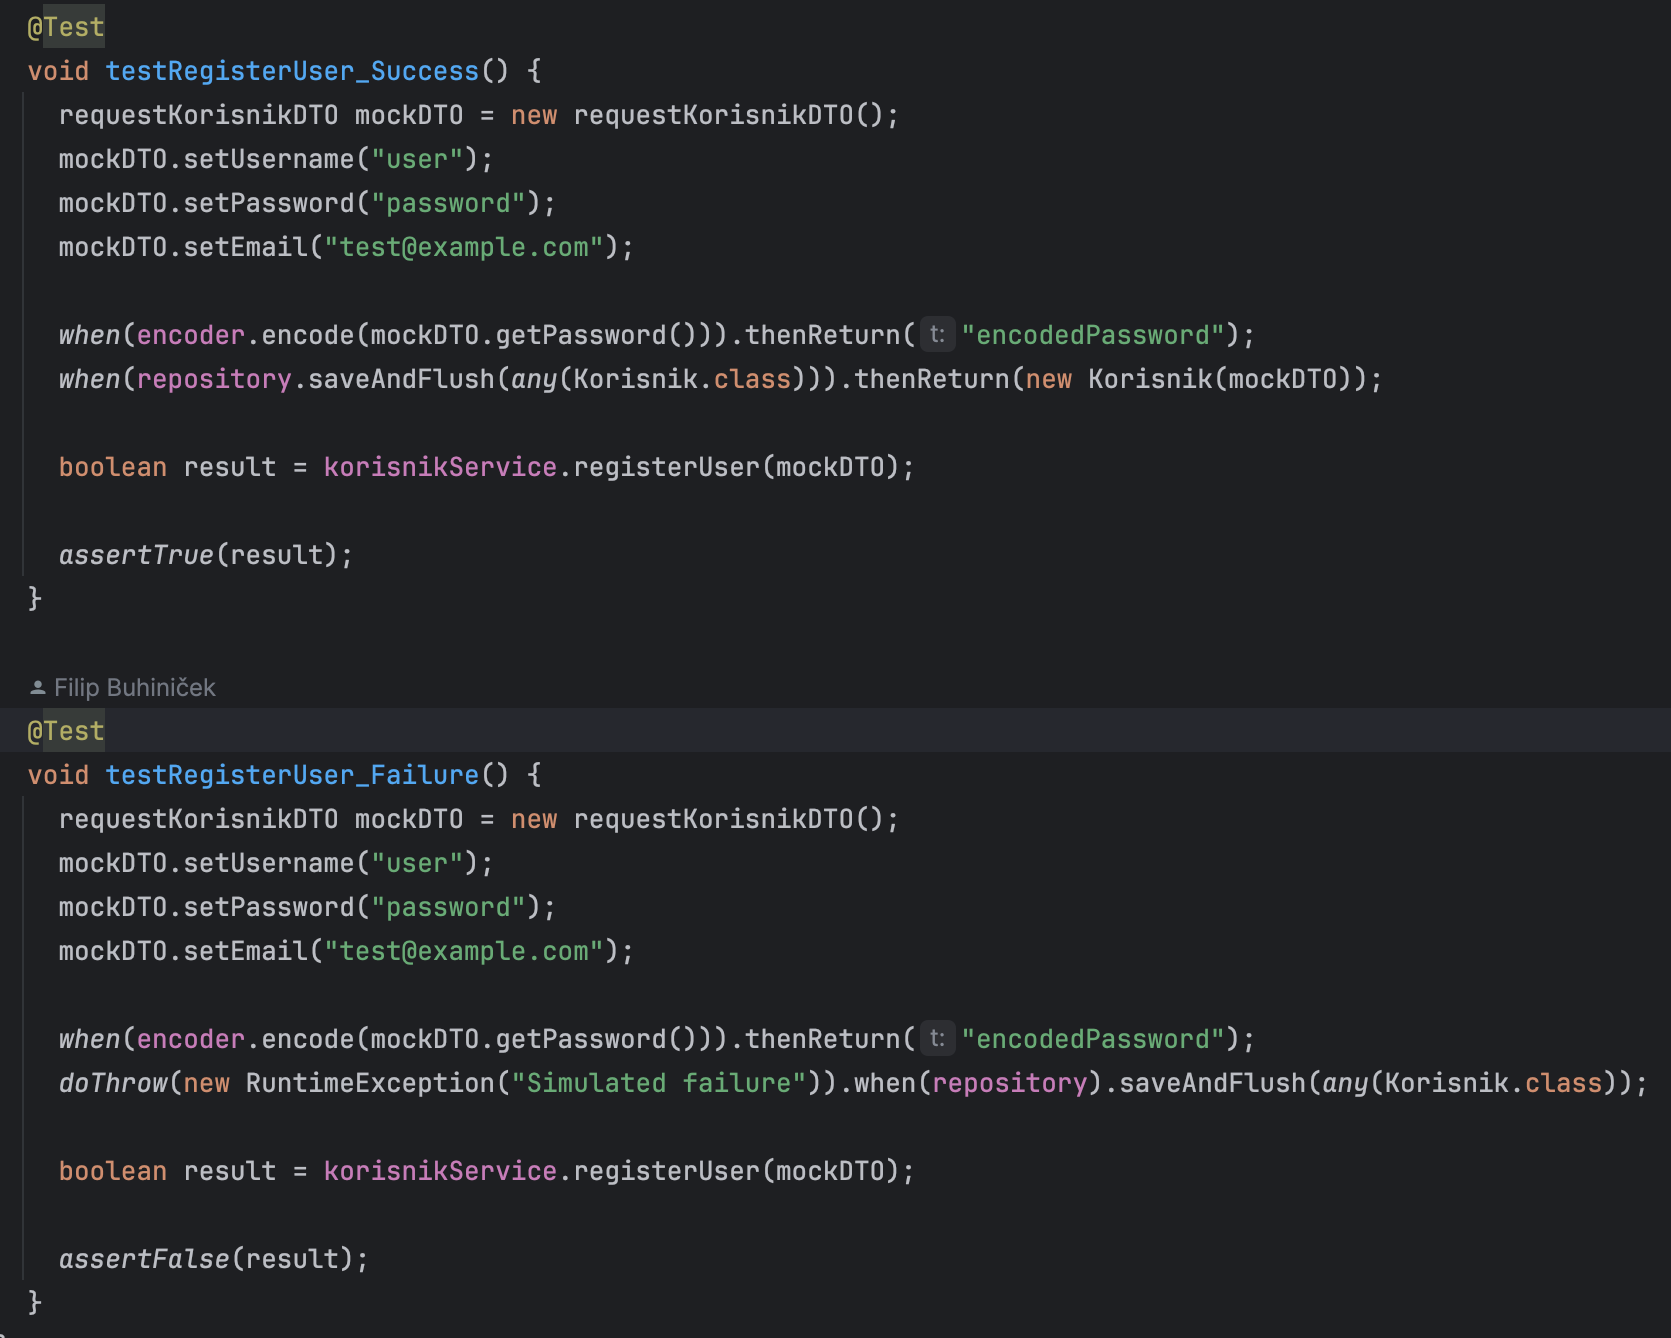
\includegraphics[scale=0.45]{testovi/korisnikTest.png}
				\centering
				\caption{Test registracije korisnika}
				\label{fig:promjene}
			\end{figure}
			
			
			
			\begin{figure}[H]
				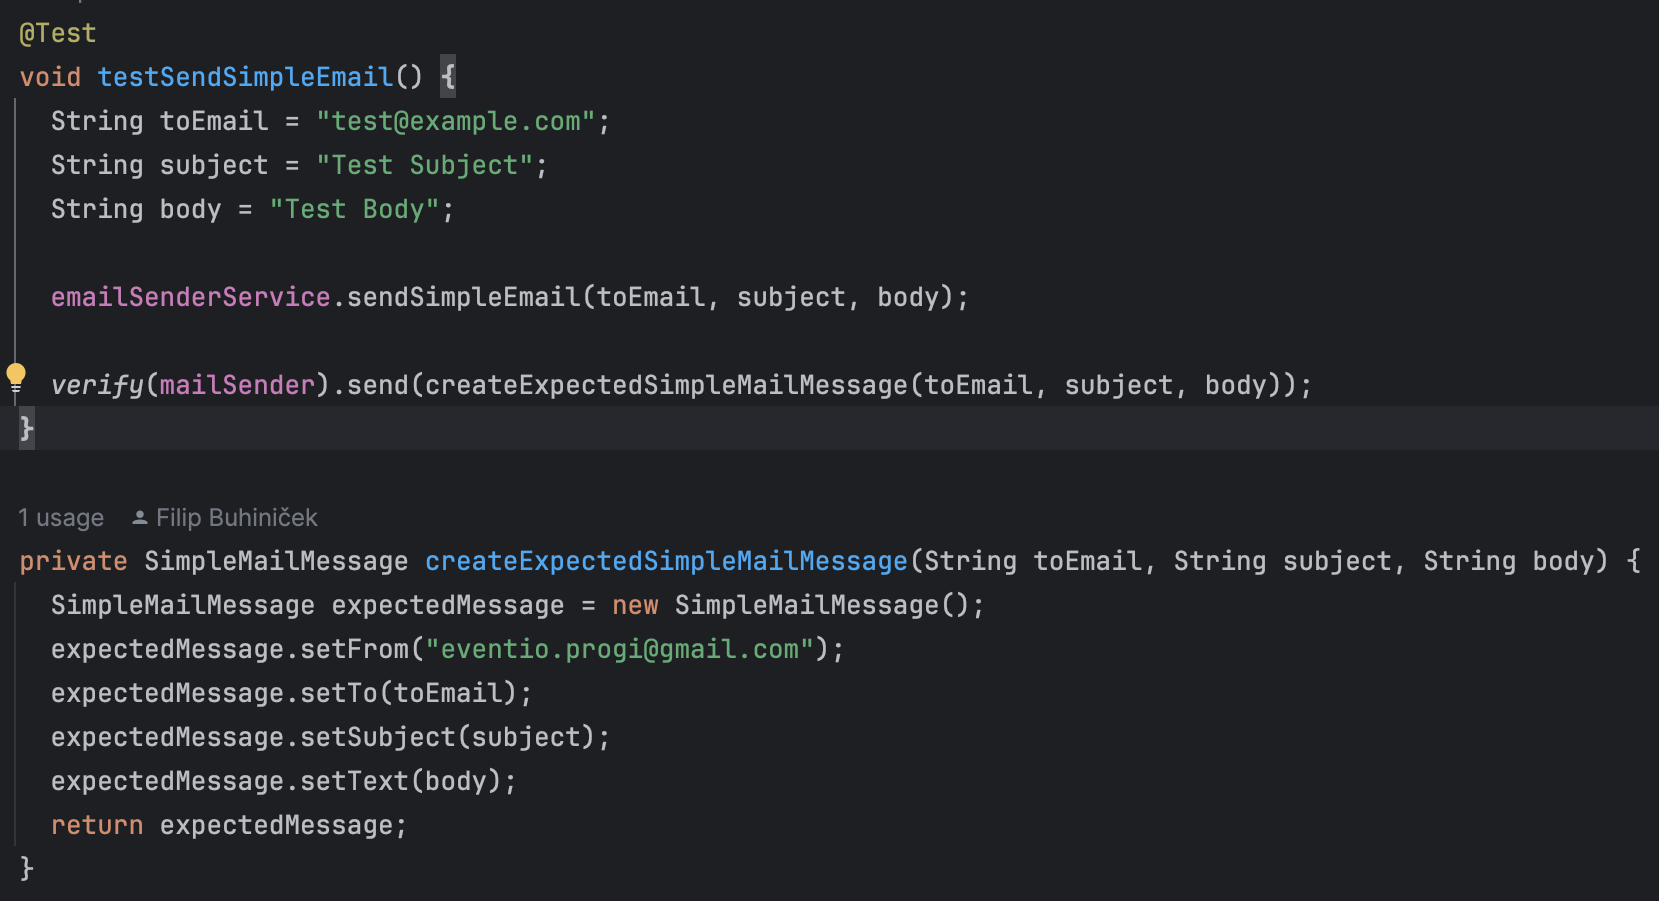
\includegraphics[scale=0.45]{testovi/emailTest.png}
				\centering
				\caption{Test slanja e-maila}
				\label{fig:promjene}
			\end{figure}
			
			\begin{figure}[H]
				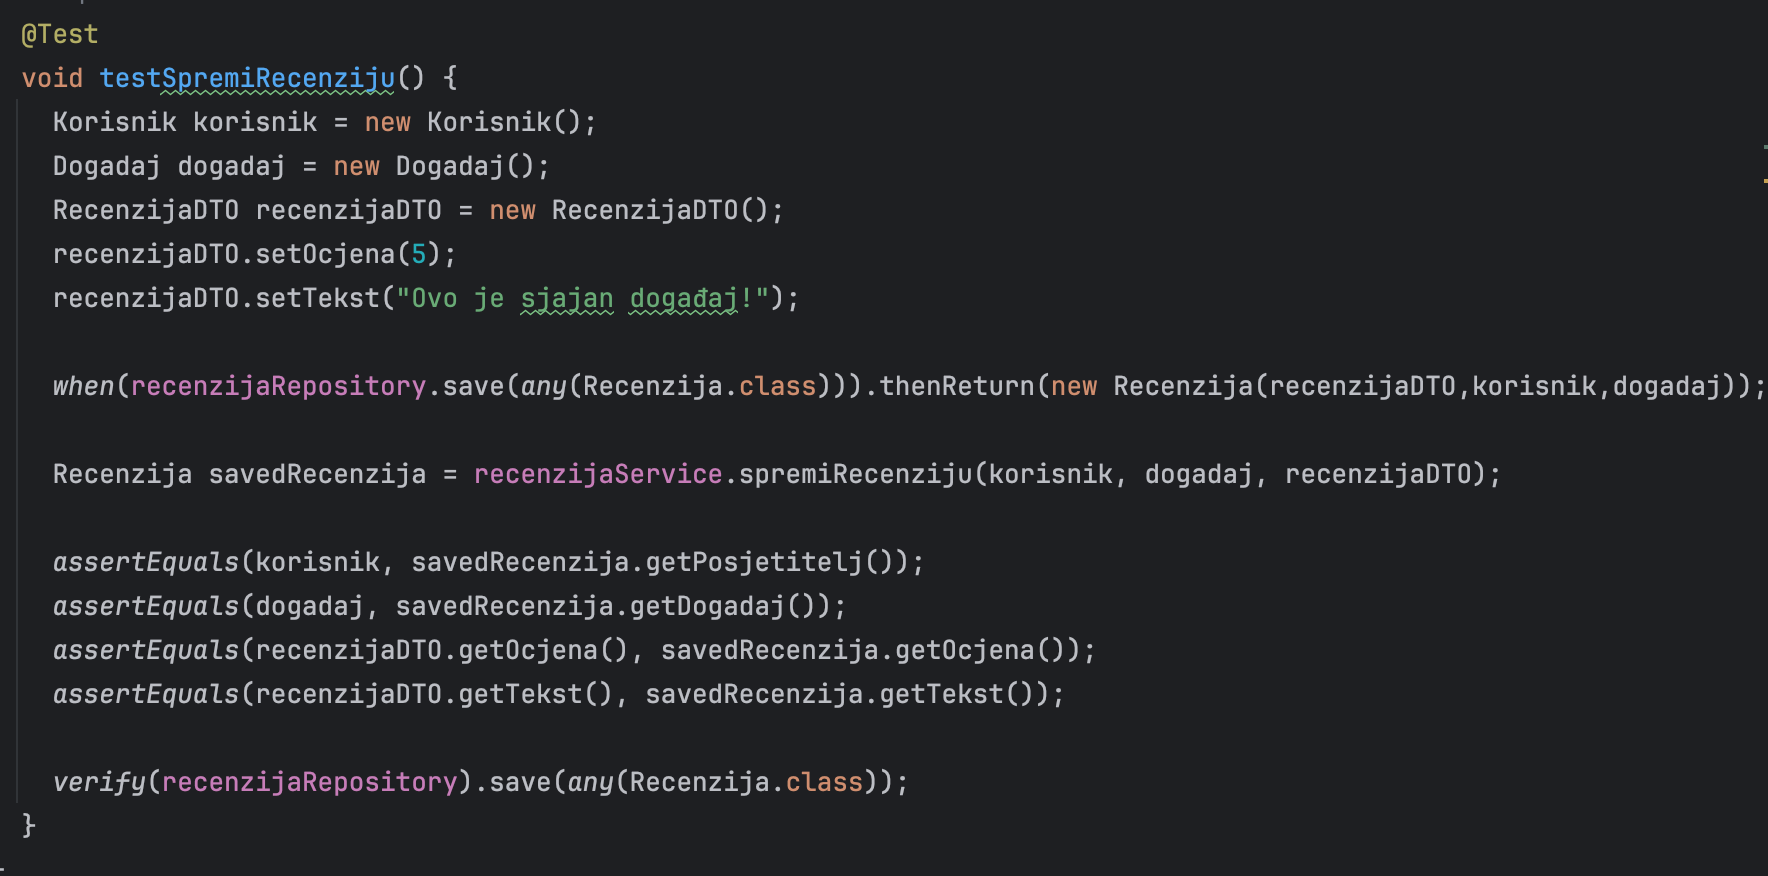
\includegraphics[scale=0.45]{testovi/recenzijeTest.png}
				\centering
				\caption{Test spremanja recenzije}
				\label{fig:promjene}
			\end{figure}
			
			\begin{figure}[H]
				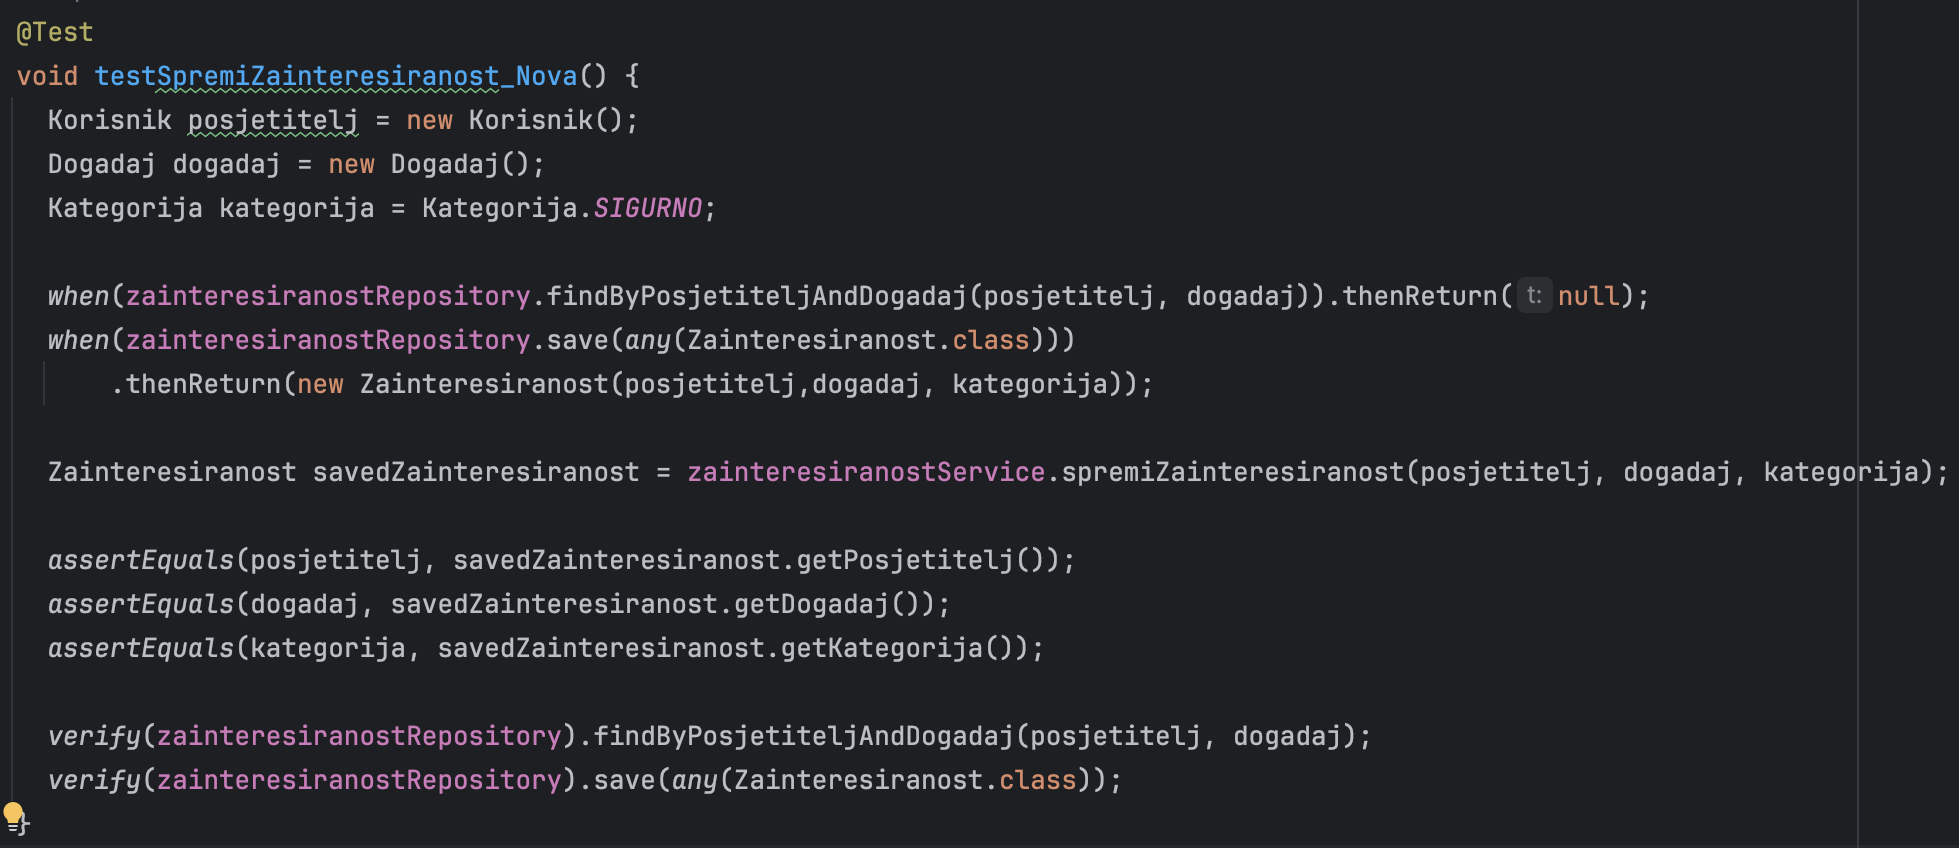
\includegraphics[scale=0.45]{testovi/zainteresiranostTest1.png}
				\centering
				\caption{Test spremanja nove zainteresiranosti}
				\label{fig:promjene}
			\end{figure}
			
			\begin{figure}[H]
				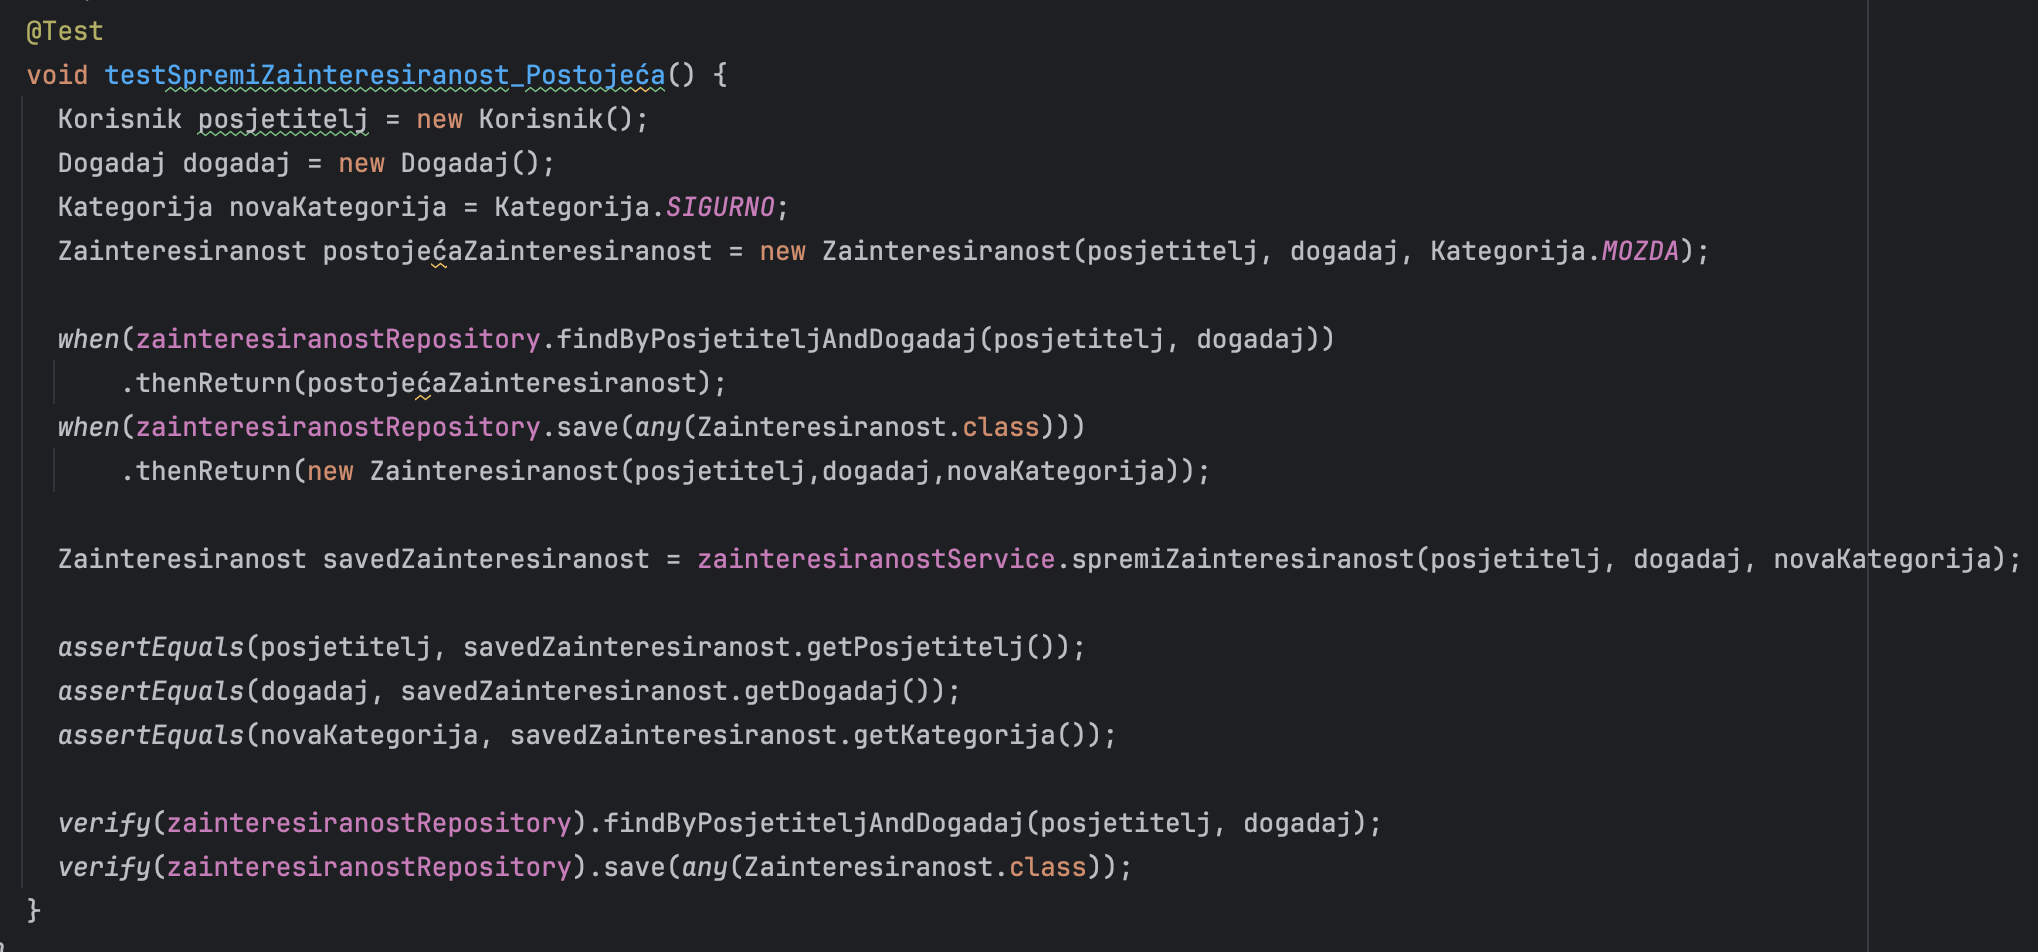
\includegraphics[scale=0.45]{testovi/zainteresiranostTest2.png}
				\centering
				\caption{Test spremanja postojeće zainteresiranosti}
				\label{fig:promjene}
			\end{figure}
			
				\begin{figure}[H]
				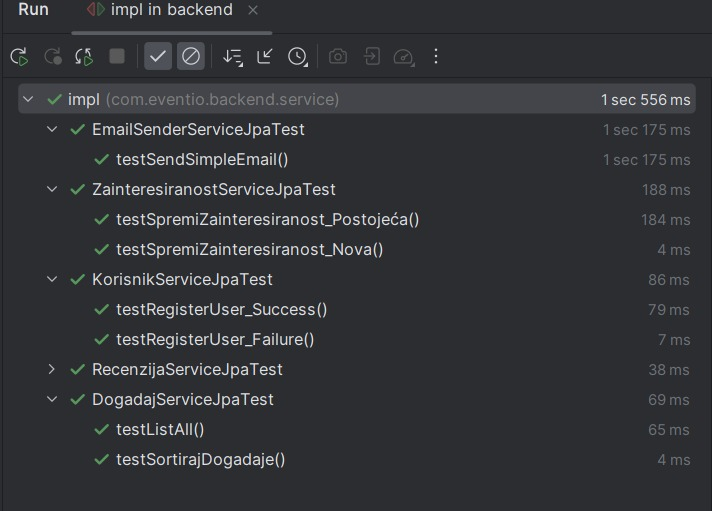
\includegraphics[scale=0.45]{testovi/unit_testovi.jpeg}
				\centering
				\caption{Izvršavanje i rezultati testova}
				\label{fig:promjene}
			\end{figure}
			
			
			\subsection{Ispitivanje sustava}
			
			U procesu ispitivanja sustava koristili smo Selenium IDE koji nam je omogućio precizno i brzo testiranje funkcionalnosti web aplikacije. Selenium IDE predstavlja moćan alat za testiranje web aplikacija te se istovremeno olakšava proces automatizacije. \newline Na sljedećim slikama prikazani su ispitni slučajevima kojima smo testirali funkcionalnost aplikacije. \textbf{Test prijave organizatora} provjerava uspješnost prijave korisnika koji je organizator. \textbf{Test stvaranja novog događaja} provjerava funkcionalnost stvaranja novog događaja sa svim postavkama. Prikazano je i izvršavanje \textbf{Testa promjene cijene pretplate} i \textbf{Testa stvaranja nove recenzije}.
			
			\begin{figure}[H]
				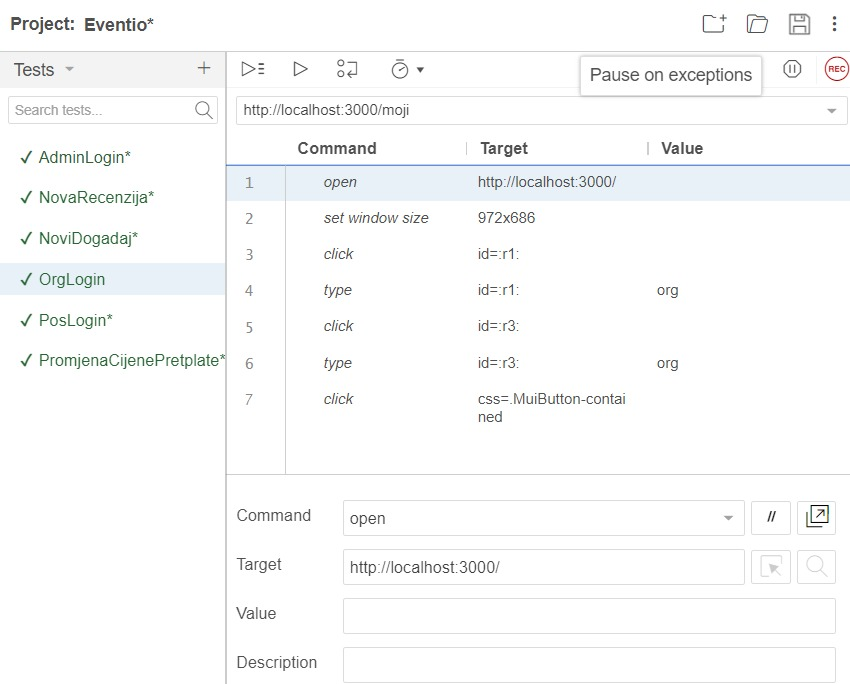
\includegraphics[scale=0.45]{testovi/selOrgLogin.jpeg}
				\centering
				\caption{Test prijave organizatora}
				\label{fig:promjene}
			\end{figure}
			
			\begin{figure}[H]
				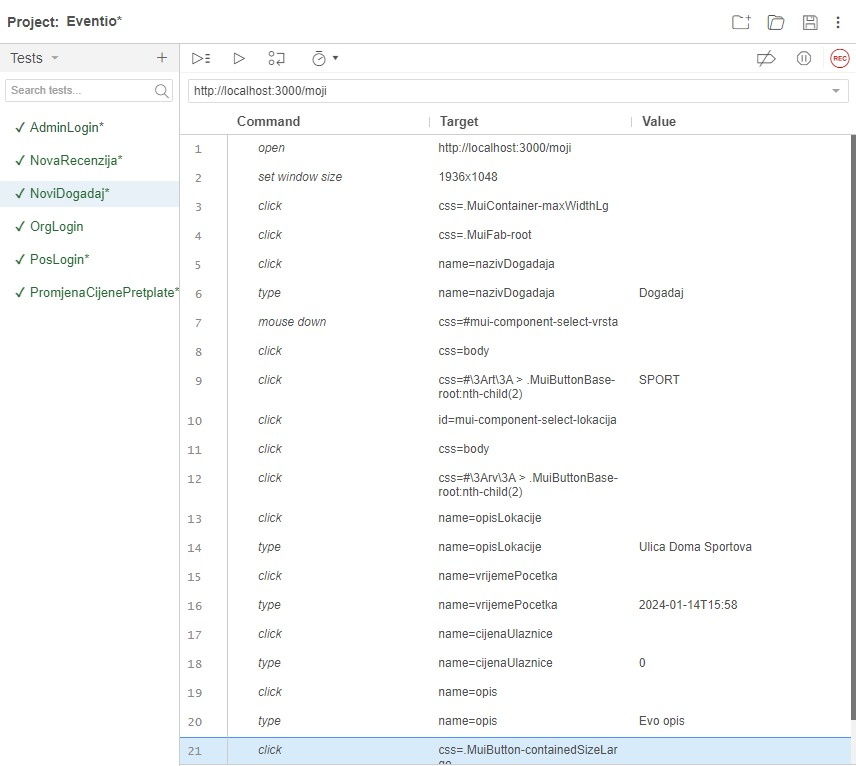
\includegraphics[scale=0.45]{testovi/selNoviDogadaj.jpeg}
				\centering
				\caption{Test stvaranja novog događaja}
				\label{fig:promjene}
			\end{figure}
			
			\begin{figure}[H]
				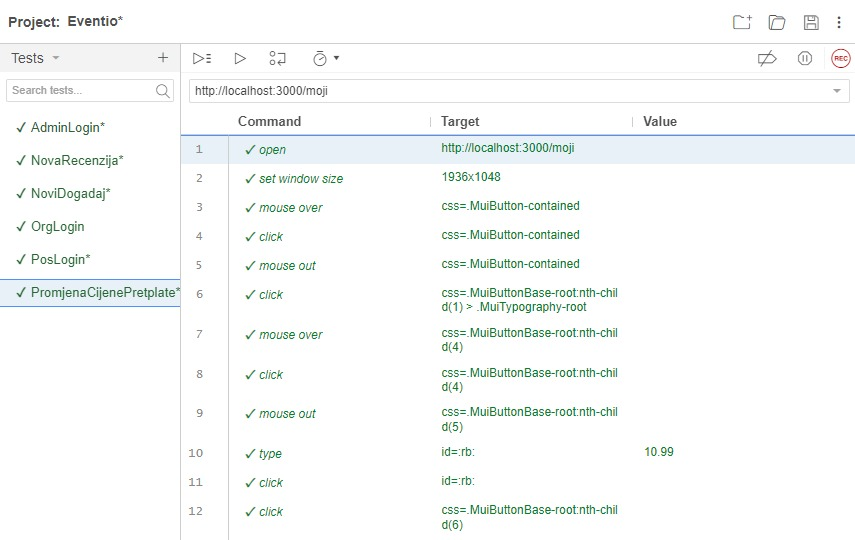
\includegraphics[scale=0.45]{testovi/selPretplata.jpeg}
				\centering
				\caption{Test promjena cijene pretplate}
				\label{fig:promjene}
			\end{figure}
			
			\begin{figure}[H]
				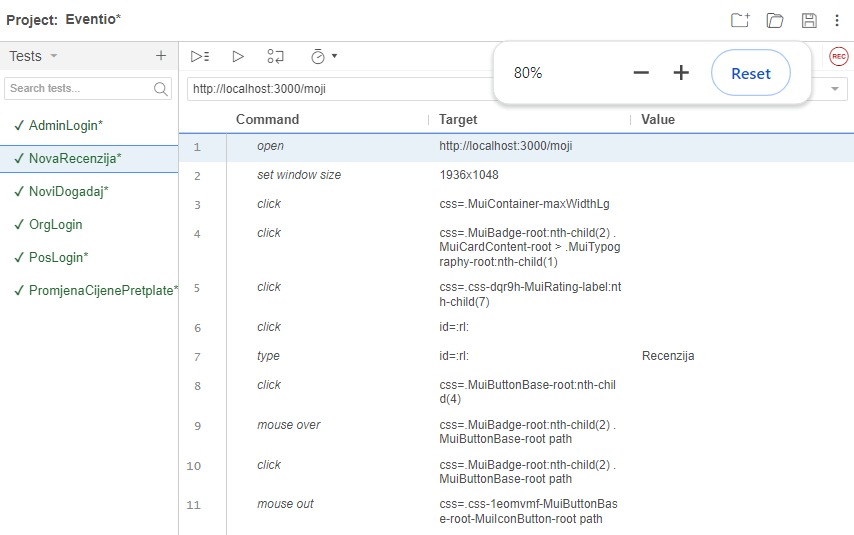
\includegraphics[scale=0.45]{testovi/selRecenzija.jpeg}
				\centering
				\caption{Test stvaranje nove recenzije}
				\label{fig:promjene}
			\end{figure}
			
		
		
		\section{Dijagram razmještaja}
			
			\textbf{\textit{dio 2. revizije}}
			
			 \textit{Potrebno je umetnuti \textbf{specifikacijski} dijagram razmještaja i opisati ga. Moguće je umjesto specifikacijskog dijagrama razmještaja umetnuti dijagram razmještaja instanci, pod uvjetom da taj dijagram bolje opisuje neki važniji dio sustava.}
			
			\eject 
		
		\section{Upute za puštanje u pogon}
		
			\textbf{\textit{dio 2. revizije}}\\
		
			 \textit{U ovom poglavlju potrebno je dati upute za puštanje u pogon (engl. deployment) ostvarene aplikacije. Na primjer, za web aplikacije, opisati postupak kojim se od izvornog kôda dolazi do potpuno postavljene baze podataka i poslužitelja koji odgovara na upite korisnika. Za mobilnu aplikaciju, postupak kojim se aplikacija izgradi, te postavi na neku od trgovina. Za stolnu (engl. desktop) aplikaciju, postupak kojim se aplikacija instalira na računalo. Ukoliko mobilne i stolne aplikacije komuniciraju s poslužiteljem i/ili bazom podataka, opisati i postupak njihovog postavljanja. Pri izradi uputa preporučuje se \textbf{naglasiti korake instalacije uporabom natuknica} te koristiti što je više moguće \textbf{slike ekrana} (engl. screenshots) kako bi upute bile jasne i jednostavne za slijediti.}
			
			
			 \textit{Dovršenu aplikaciju potrebno je pokrenuti na javno dostupnom poslužitelju. Studentima se preporuča korištenje neke od sljedećih besplatnih usluga: \href{https://aws.amazon.com/}{Amazon AWS}, \href{https://azure.microsoft.com/en-us/}{Microsoft Azure} ili \href{https://www.heroku.com/}{Heroku}. Mobilne aplikacije trebaju biti objavljene na F-Droid, Google Play ili Amazon App trgovini.}
			
			
			\eject 